\newpage
\section{Навчання з підсиленням (reinforcement learning)}

\subsection{Короткий вступ}

\emph{Навчання з підсиленням (Reinforcement learning)} - навчання про те, які дії потрібно приймати залежно від ситуації таким чином, щоб максимізувати \emph{числовий сигнал "винагороди" (reward signal)}. ``Учневі'' не вказується, які дії потрібно здійснювати, щоб досягти мети, а натомість дається можливість самому вибирати з певного набору допустимих дій. В результаті багаторазової взаємодії з середовищем шляхом методу спроб та помилок досягається оптимальна ``стратегія'' (послідовність дій, які ведуть до мети).

У загальному випадку, вибрані дії впливають не тільки на винагороду, що слідує безпосередньо після вчинення дії, але й на майбутні ситуації, що, в свою чергу, дає вплив на мабутні винагороди.

В навчанні з підсиленням присутні дві сутності "--- агент та середовище. Агент "--- це все те, на що ми можемо чинити безпосередній вплив.
Накриклад, якщо ми маємо робота, то агентом може бути як весь робот, якщо ми здатні безпосередньо керувати його поворотом навколо своєї осі. Або агентом можна визначити лише електромотори, які зумовлюють поворот коліс та їх рух. В останньому випадку ми безпосередньо можемо впливати тільки на силу струму, що подається на електромотори. На самі ж колеса ми впливаємо опосередковано, тому вони вважаються середовищем, по відношенню до нашого агента.

Стан системи "--- набір параметрів, які задають наші знання (можливо неповні) про оточуючий світ в конкретний момент часу. Це, фактично, наше сприйняття поточної ситуації. Наприклад, у випадку автономного керування транспортним засобом, станом буде інформація про
відстань до найближчої перешкоди, відстань до заданої цілі, можливо, поточна швидкість самого транспортного засобу тощо.

Складовими частинами системи навчання з підсиленнями є:
\begin{itemize}
\item \emph{Стратегія (policy)}, яка визначає те, які дії будуть прийматися
залежно від ситуації на даний момент часу. Стратегія "--- це, фактично, інтелект агента.
\item \emph{Функція винагороди (reward function)}, яка задає відображення зі стану системи та здійсненої дії у множину дійсних чисел "--- множину винагород. Тобто після кожної здійсненої дії, залежно від стану системи, агент отримує певне миттєве значення винагороди. Глобальною метою агента є максимізація загальної винагороди, отриманої протягом всього часу його дії.
\item \emph{Вартісна функція (value function)}, яка, на відміну від функції винагороди, задає не те, що є ``корисним'' безпосередньо зараз, а те, що є корисним в більш глобальному значенні: з урахуванням майбутніх станів.
\end{itemize}

Розглянемо ці поняття більш формально, базуючись на інформації з \cite{SuttonBarto2002}.

\subsection{Модель навчання з підсиленням}

\emph{Агент (agent)} та \emph{середовище (environment)} взаємодіють в кожен дискретний момент часу $t=0,1,2,\dots$. На кожному кроці $t$ агент отримує певне представлення \emph{стану системи (state)} $s_t \in \mathcal{S}$, де $\mathcal{S}$ "--- множина усіх станів системи, і на базі цього вибирає \emph{дію (action)} $a_t \in \mathcal{A}(s_t)$, де $\mathcal{A}(s_t)$ "--- множина допустимих дій у стані $s_t$. На наступному кроці $t+1$, частково як наслідок виконаної дії, агент отримує числову \emph{винагороду (reward)} $r_{t+1} \in \mathbb{R}$ і опиняється в стані $s_{t+1}$.

\begin{figure}[!h]
\centering
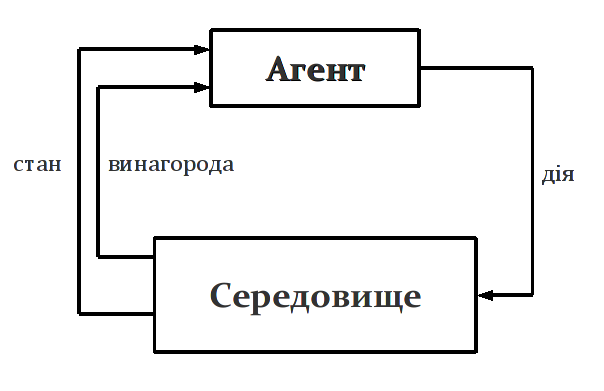
\includegraphics[width=0.7\textwidth]{agent_env_diagram.png}
\caption{Взаємодія агента та середовища в навчанні з підсиленням.}
\end{figure}

В загальному випадку, на кожному кроці агент реалізовує відображення станів системи на ймовірності здійснення можливої дії. Таке відображення називається \emph{стратегією (policy)} агента і позначається $\pi_t$, де $\pi_t(s,a)$ "--- це ймовірність, що $a_t=a$, якщо $s_t = s$.
%У випадку детермінованої стратегії:
%\[
%    \pi_t(s,a) = \begin{cases}
%                     1, & \textrm{якщо } s=s_t \textrm{ і } a=a_t \\
%					 0, & \textrm{інакше}
%                 \end{cases}
%\]

Методи навчання з підсиленням визначають, як саме агент змінює свою стратегію в результаті набутого досвіду. Мета агента, грубо кажучи,"--- максимізувати сукупну винагороду, яку він отримує протягом багатьох ходів.

\subsection{Прибуток (return)}

Визначимо більш точно мету агента. Нехай, починаючи з часу $t$, агент отримує послідовність винагород $r_{t+1}, r_{t+2}, r_{t+3}, \ldots$. Тоді основною метою агента буде максимізація \emph{очікуваного прибутку (expected return)} $R_t$, де $R_t$ "--- це певна функція від послідовності винагород. В найпростішому випадку прибуток є сумою усіх винагород:

\begin{equation}
R_t = r_{t+1} + r_{t+2} + \cdots + r_T,
\end{equation}
де $T$ "--- кінцевий момент часу. Такий підхід до визначення прибутку підходить там, де можна природно визначити фінальний момент часу, тобто в таких системах, в яких взаємодія агента і середовища природньо розбивається на окремі послідовності (\emph{епізоди}), наприклад, партії в грі, проходи по лабіринту або будь-який інший вид повторюваних взаємодій.

Кожен епізод закінчується у \emph{кінцевому (термінальному) стані (terminal state)}, після якого відбувається встановлення стану системи в певний початковий стан з множини можливих початкових станів і розпочинається наступний епізод. Задачі, в яких взаємодія агента і середовища відбувається у вигляді послідовності епізодів, називаються \emph{епізодичними задачами (episodic tasks)}. В епізодичних задачах інколи розмежовують множину усіх нетермінальних станів системи $\mathcal{S}$ та множину усіх станів, включно з термінальними $\mathcal{S^+}$.

З іншого боку, не завжди можна здійснити природній поділ на епізоди, натомість взаємодія відбуваєть постійно без закінчення. Прикладом такої задачі може бути діяльність робота з великою тривалістю життєдіяльності. Такі задачі назвемо \emph{неперервними задачами (continuing tasks)}. В такому випадку кінцевий момент часу $T=\infty$, а сам прибуток, який ми намагаємося максимізувати може легко прямувати до нескінченості (наприклад, якщо на кожному кроці $r_t=1$). Щоб подолати ці труднощі, введемо дещо інше визначення прибутку.

Розглянемо додаткову концепцію "--- \emph{дисконтування (discounting)}. Згідно з нею, агент намагаєтсья вибирати такі дії, щоб максимізувати суму дисконтованих винагород, які він отримає в майбутньому. Зокрема, агент вибирає таку дію $a_t$, яка максимізує очікуваний \emph{дисконтований прибуток (discounted reward)}:

\begin{equation}
R_t = r_{t+1} + \gamma r_{t+2} + \gamma^2 r_{t+3} + \cdots = \sum_{k=0}^{\infty}\gamma^k r_{t+k+1},
\end{equation}
де $\gamma$ "--- це параметр, який називається \emph{дисконтною ставкою (discount rate)}, $0\leq\gamma\leq 1$.

Дисконтна ставка визначає поточну вагу майбутньої винагороди: винагорода, отримана через $k$ кроків у майбутньому, має вагу лише $\gamma^k$, напротивагу одиничній вазі, яку б вона мала, якби була отримана на поточному кроці. Якщо $\gamma<1$, то ця нескінченна сума має скінченне значення, якщо послідовність $\left\{r_k\right\}$ "--- обмежена. Якщо $\gamma = 0$, то агент є ``недалекоглядним'' і буде дбати лише про максимізацію миттєвої винагороди. Його задачею в такому випадку буде вибір такої дії $a_t$, щоб максимізувати лише винагороду $r_{t+1}$. Якщо дія агента не здійснює вплив на майбутні винагороди, то такий підхід дійсно дасть змогу вивчити оптимальну стратегію, однак в більшості випадків це не так, тому максимізація лише миттєвої нагороди може призвести до того, що буде втрачено нагоду ``заробити'' більше в майбутньому, здійснивши на даному кроці дію, яка принесе не максимальну миттєву винагороду. З наближенням $\gamma$ до 1, агент буде надавати майбутнім винагородам все більшого значення: агент стає більш ``далекоглядним''.

\subsection{Функція корисності (value function)}

Практично всі алгоритми навчання з підсиленням базуються на оцінці \emph{функції корисності (value function)} "--- функції станів системи (або пари стан-дія), що оцінює \emph{наскільки добре} для агента перебувати в заданому стані (або наскільки добре здійснити задану дію, перебуваючи в заданому стані). Фраза ``наскільки добре'' визначається в термінах майбутніх винагород або, що є точнішим визначенням, в термінах очікуваного майбутнього прибутку. Очевидно, що майбутні винагороди залежать від того, які дії здійснювати, тобто від стратегії, тому ціннісна функція визначається з врахуванням певної стратегії.

Нагадаємо, що стратегія $\pi$ "--- це відображення кожного стану $s \in \mathcal{S}$ та кожної допустимої дії $a \in \mathcal{A}(s)$ на ймовірність $\pi(s,a)$ здійснення дії $a$, будучи в стані $s$. \emph{Корисністю} стану $s$ згідно стратегії $\pi$, $V^\pi(s)$,"--- це очікуваний прибуток, який можна отримати, якщо почати зі стану $s$ і діяти згідно стратегії $\pi$:
\begin{equation}
V^\pi(s) = E_\pi \Bigl\{ R_t \Big| s_t = s \Bigr \} = E_\pi \Biggl\{\sum_{k=0}^{\infty}\gamma^k r_{t+k+1} \Bigg| s_t=s \Biggr\},
\end{equation}
де $E_\pi{}$ позначає математичне очікування в випадку, якщо агент діє згідно стратегії $\pi$. Потрібно відмітити, що цінність термінального стану завжди рівна нулю. Назвемо функцію $V^\pi$ \emph{функцією корисності станів (state-value function) для статегії $\pi$}.

Аналогічно, визначимо корисність здійснення дії $a$ в стані $s$ згідно стратегії $\pi$, $Q^\pi(s,a)$, як очікуваний прибуток, отриманий в результаті перебування в стані $s$, здійснення дії $a$ та подальшому слідуванні стратегії $\pi$:
\begin{equation}
Q^\pi(s,a)=E_\pi \Bigl\{ R_t \Big| s_t=s, a_t=a \Bigr\} = E_\pi \Biggl\{\sum_{k=0}^{\infty}\gamma^k r_{t+k+1} \Bigg| s_t=s,a_t=a \Biggr\}.
\end{equation}
Назвемо функцію $Q^\pi$ \emph{функцією корисності дій (action-value function) для статегії $\pi$}.

Функції корисності $V^\pi$ та $Q^\pi$ можуть бути оцінені з досвіду. Наприклад, якщо агент притримується стратегії $\pi$ і підтримує середнє значення всіх прибутків, які були реально отримані, для кожного стану, в якому перебував агент, то середнє значення збіжиться до значення цінності для даного стану $V^\pi(s)$ за умови, що кількість перебувань в кожному зі станів прямує до нескінченності. Якщо зберігати середні значення окремо для кожної пари стан-дія, то таке ж твердження вірне і для функції $Q^\pi$. Такі методи оцінки цінових функцій називаються \emph{методами Монте-Карло}, тому що вони використовують усереднення по випадкових прикладах реальних прибутків. Проте, якщо кількість станів та можливих дій велика, це унеможливлює збереження середніх значень для кожного стану (пари стан-дія). В такому випадку можна застосувати інші методи, зокрема такі, що використовують апроксиматори функцій. Ми розглянемо їх дещо пізніше.

Фундаментальна властивість функцій корисності, яка використовується в навчанні з підсиленням і динамічному програмуванні,"--- це певне рекурсивне співвідношення, якому задовільняє функція корисності. Для будь-якої фіксованої стратегії $\pi$ та будь-якого стану $s$, наступне співвідношення завжди виконується:
\begin{eqnarray}
V^\pi(s) & = & E_\pi \Bigl\{R_t \Big| s_t = s \Bigr\} \nonumber\\
			& = & E_\pi \Biggl\{\sum_{k=0}^{\infty}\gamma^k r_{t+k+1} \Bigg| s_t = s \Biggr\} \nonumber\\
			& = & \sum_a \pi(s,a)\sum_{s'}\mathcal{P}^a_{ss'} \left[ \mathcal{R}^a_{ss'}+\gamma E_\pi \left\{\sum_{k=0}^{\infty}\gamma^k r_{t+k+2} \Bigg| s_{t+1} = s' \right\} \right] \nonumber\\
			& = & \sum_a \pi(s,a)\sum_{s'}\mathcal{P}^a_{ss'} \left[ \mathcal{R}^a_{ss'}+\gamma V^\pi(s') \right],
\label{Bellman_eq}
\end{eqnarray}
де $\mathcal{P}^a_{ss'}$ "--- це ймовірність переходу (transition probability) зі стану $s$ в стан $s'$ при виконанні дії $a$; $\mathcal{R}^a_{ss'}$ "--- очікувана винагорода, яка дається агенту при переході зі стану $s$ в стан $s'$ при виконанні дії $a$. В даній формулі неявно розуміється, що $s \in \mathcal{S}$, дії $a$ беруться з множини $\mathcal{A}(s)$, а $s' \in \mathcal{S}$ у випадку неперервної задачі або $s' \in \mathcal{S^+}$ "--- у випадку епізодичної задачі. Вказані ймовірності та очікувані винагороди визначають повну динаміку системи і на практиці зазвичай не відомі. Тому доводиться шукати методи, які б не потребували повних знань про систему.

Рівняння (\ref{Bellman_eq}) називається \emph{рівнянням оптимальності Белмана для $V^\pi$ (Bellman optimality equation for $V^\pi$)}. Воно відображає зв'язок між корисністю стану $s$ та корисністю станів $s'$, в які можна потрапити з $s$. Можна довести, що функція $V^\pi$ "--- єдиний розв'язок рівняння Белмана. Відмітимо також, що це рівняння "--- основа для багатьох методів обчислення, наближення та вивчення $V^\pi$.

\subsection{Оптимальні функції корисності}

Розв'язування задачі навчання з підсиленням означає, згрубша, знаходження такої стратегії, яка б давала великий прибуток в довгостроковій перспективі. Спробуємо визначити оптимальність стратегії наступним чином. Функції корисності визначають частковий порядок на множині усіх стратегій. Стратегію $\pi$ називатимемо \emph{кращою}, ніж стратегія $\pi '$, якщо її очікуваний прибуток більший або рівний від такого ж для стратегії $\pi '$ для усіх станів $s \in \mathcal{S}$:
\begin{equation}
\pi \geq \pi ' \Leftrightarrow \Bigl(\forall s \in \mathcal{S}\Bigr)\left\{ V^\pi(s) \geq V^{\pi '}(s) \right\}
\end{equation}

Завжди існує хоча б одна така стратегія, яка краща або рівна, ніж усі інші. Така стратегія називається \emph{оптимальною}. Хоча оптимальних стратегій може бути декілька, всіх їх будемо позначати як $\pi^*$. Усі оптимальні стратегії мають одну і ту ж функцію корисності станів, яка називається \emph{оптимальною функцією корисності станів} $V^*$:
\begin{equation}
V^* = \max_\pi V^\pi(s),\qquad \forall s \in \mathcal{S}.
\end{equation}

Оптимальні стратегії також мають одну і ту ж \emph{функцію корисності дій} $Q^*$:
\begin{equation}
Q^* = \max_\pi Q^\pi(s,a),\qquad \forall s \in \mathcal{S}, \forall a \in \mathcal{A}(s).
\end{equation}

Ми можемо також записати функцію $Q^*$ в термінах $V^*$:
\begin{equation}
Q^*(s,a) = E\left\{r_{t+1} + \gamma V^*(s_{t+1}) \Big| s_t=s, a_t=a \right\}.
\end{equation}

\section{Методи розв'язування задач навчання з підсиленням}

Існує три широких класи методів, призначених для розв'язування задач навчання з підсиленням:
\begin{itemize}
\item методи динамічного програмування (dynamic programming methods);
\item методи Монте-Карло (Monte Carlo methods);
\item метод часової різниці (temporal-difference learning).
\end{itemize}

Кожен з цих класів має свої сильні та слабкі сторони. Так, методи динамічного програмування є добре розробленими з математичної точки зору, але потребують повної і достатньо точної моделі середовища, що часто просто неможливо задовільнити. Методи Монте-Карло не потребують моделі середовища і є концептуально простими, проте вони не є пристосованими до покрокових послідовних обчислень. Методи ж навчання з часовою різницею не потребують моделі середовища і добре пристосовані до послідовних покрокових обчислень, але є складнішими для аналізу. Ці методи також відрізняються в плані ефективності та швидкості збіжності.

В даній роботі був використаний саме останній метод, на якому зупинимося більш детально.

\subsection{Навчання з часовою різницею (TD-методи)}

Ідея методів \emph{навчання з часовою різницею (temporal-difference, TD-навчання)} є, мабуть, центральною та найбільш новаторською для всього навчання з підсиленням. TD-навчання "--- це поєднання ідей методів Монте-Карло та динамічного програмування. TD-методи можуть, як і методи Монте-Карло, навчатися лише з досвіду, не потребуючи знання моделі динаміки середовища. З іншого боку, так само як і в методах динамічного програмування, TD-методи оновлюють свої оцінки частково на основі інших оцінок, не чекаючи закінчення епізоду. Така оцінка на базі інших оцінок отримала назву \textit{``стартування'' (bootstrap)}.

\subsubsection{TD-прогнозування}

Як TD, так і Монте-Карло методи використовують отриманий досвід для розв'язування задачі прогнозування. Маючи певний досвід, отриманий в результаті притримування стратегії $\pi$, обидва методи використовують його для оновлення наближення $V$ до $V^\pi$. Якщо в момент часу $t$ був відвіданий нетермінальний стан $s_t$, то обидва методи оновлять свої наближення $V(s_t)$, базуючись на тому, що відбудеться в наступні моменти часу. Так, метод Монте-Карло чекає моменту, коли стане відомим прибуток, отриманий після відвідання поточного стану, а тоді використовує цей прибуток як наближення для $V(s_t)$. Простий алгоритм Монте-Карло для всіх візитів (every-visit Monte Carlo) виглядає наступним чином:
\begin{equation}
V(s_t) \leftarrow V(s_t) + \alpha\left[R_t - V(s_t)\right],
\end{equation}
де $R_t$ "--- реальний прибуток, отриманий протягом поточного епізоду, починаючи з моменту часу $t$, $\alpha$ "--- сталий параметр величини кроку.

В той час, як MC-метод чекає до закінчення епізоду, TD-метод повинен чекати лише наступного моменту часу. В момент $t+1$ алгоритм формує наближення на основі отриманої винагороди $r_{t+1}$ та наближення $V(s_{t+1})$. Найпростіший TD-алгоритм, знаний як TD(0), виглядає наступним чином:
\begin{equation}
V(s_t) \leftarrow V(s_t) + \alpha\left[r_{t+1} + \gamma V(s_{t+1}) - V(s_t)\right].
\end{equation}

Раніше вже згадувалося, що
\begin{eqnarray}
V^\pi(s) & = & E_\pi \Bigl\{R_t \Big| s_t = s \Bigr\} \label{MC_target}\\
			& = & E_\pi \Biggl\{\sum_{k=0}^{\infty}\gamma^k r_{t+k+1} \Bigg| s_t = s \Biggr\} \nonumber\\
			& = & E_\pi \left\{r_{t+1} + \gamma\sum_{k=0}^{\infty}\gamma^k r_{t+k+2} \Bigg| s_t = s \right\} \nonumber\\
			& = & E_\pi \left\{r_{t+1} + \gamma V^\pi(s_{t+1}) \bigg| s_t = s \right\}.\label{DP_target}
\end{eqnarray}

Таким чином, з попереднього запису видно, що MC-метод використовує наближення з (\ref{MC_target}) як бажане значення ціннісної функції, а DP-метод "--- з (\ref{DP_target}). Бажане значення для MC є наближенням, оскільки невідоме математичне сподівання. В випадку з DP воно є наближенням не через матсподівання, яке відоме з моделі динаміки середовища, а через те, що саме значення $V^\pi(s_{t+1})$ невідоме. Для TD-методу ми ж отримуємо наближення і через невідомість матсподівання, і через невідомість реального значення $V^\pi(s_{t+1})$. В табл.~\ref{TD0_algorithm} поданий алгоритм TD(0).

\begin{table}
\centering
\begin{tabular}{|l|}
\hline\\
Ініціалізувати $V(s)$ довільним значенням\\
Ініціалізувати $\pi$ стратегією, яка відповідає згенерованій $V(s)$\\
Для кожного епізоду повторювати:\\
\hspace{0.5cm} Ініціалізувати $s$\\
\hspace{0.5cm} Повторювати для кожного кроку епізоду:\\
\hspace{1cm} 	$a \leftarrow $ дія, пропонована поточною стратегією $\pi$ для стану $s$\\
\hspace{1cm} 	Виконати дію $a$; спостерегти винагороду $r$ та наступний стан $s'$\\
\hspace{1cm} 	$V(s) \leftarrow V(s) + \alpha\left[r + \gamma V(s') - V(s)\right]$\\
\hspace{1cm} 	$s \leftarrow s'$\\
\hspace{0.5cm} поки $s$ "--- нетермінальний стан\\
\\
\hline
\end{tabular}
\caption{Алгоритм TD(0) для наближення $V^\pi$.}
\label{TD0_algorithm}
\end{table}

\subsubsection{Алгоритм Sarsa}

Розглянемо тепер застосування TD-алгоритмів до задачі контролю. Натомість функції корисності станів ми будемо намагатися вивчити функцію корисності стану-дії $Q^\pi(s,a)$. Нагадаємо, що епізод складається з почергової послідовності станів та пар стан-дія:
\begin{figure}
\centering
\begin{picture}(400,100)
	\Large
	\thicklines
    \multiput(20,50)(130,0){3}{\circle{40}}
	\multiput(40,50)(130,0){3}{\line(1,0){40}}
    \multiput(85,50)(130,0){3}{\circle*{10}}
	\multiput(90,50)(130,0){2}{\line(1,0){40}}
	\put(340,50){\line(1,0){25}}
	\put(375,50){\line(1,0){3}}
	\put(382,50){\line(1,0){3}}
	\put(389,50){\line(1,0){3}}
	\put(15,47){$\displaystyle s_t$}
	\put(138,47){$\displaystyle s_{t+1}$}
	\put(266,47){$\displaystyle s_{t+2}$}

	\put(70,33){$\displaystyle s_t,a_t$}
	\put(187,33){$\displaystyle s_{t+1},a_{t+1}$}
	\put(313,33){$\displaystyle s_{t+2},a_{t+2}$}
	\put(100,60){$\displaystyle r_{t+1}$}
	\put(227,60){$\displaystyle r_{t+2}$}
\end{picture}
\caption{Послідовність подій в Sarsa}
\label{sarsa_diagram}
\end{figure}

%\begin{center}\includegraphics[width=0.7\textwidth]{sarsa_diagram.png}\end{center}

Раніше ми розглядали переходи зі стану в стан і вивчення цінності станів. Тепер ми будемо розглядати переходи між парами стан-дія і вивчення цінності стану-дії. Відповідне правило навчання виглядає наступним чином:
\begin{equation}
Q(s_t,a_t) \leftarrow Q(s_t,a_t) + \alpha\left[r_{t+1} + \gamma Q(s_{t+1},a_{t+1}) - Q(s_t, a_t)\right].
\end{equation}

Це оновлення робиться після кожного переходу з нетермінального стану $s_t$. Якщо $s_{t+1}$ "--- термінальний стан, то $Q(s_{t+1}, a_{t+1})$ визначається рівним нулю. Це правило використовує кожен елемент з п'ятірки подій, $(s_t,a_t,r_{t+1},s_{t+1},a_{t+1})$ (рис.~\ref{sarsa_diagram}), що становлять перехід з однієї пари стан-дія в іншу. Ця п'ятірка і дала назву алгоритму "--- \emph{Sarsa}.

\begin{table}
\centering
\begin{tabular}{|l|}
\hline\\
Ініціалізувати $Q(s,a)$ довільним чином\\
Для кожного епізоду повторювати:\\
\hspace{0.5cm} Ініціалізувати $s$\\
\hspace{0.5cm} Обрати $a$ зі стану $s$ згідно стратегії, що базується на $Q$ (наприклад, $\varepsilon$-жадібну)\\
\hspace{0.5cm} Повторювати для кожного кроку епізоду:\\
\hspace{1cm} 	Здійснити дію $a$, спостерегти $r$, $s'$\\
\hspace{1cm} 	Обрати $a'$ зі стану $s'$ згідно стратегії\\
\hspace{1cm} 	$Q(s,a) \leftarrow Q(s,a) + \alpha\left[r + \gamma Q(s',a') - Q(s,a)\right]$\\
\hspace{1cm} 	$s \leftarrow s';\ a \leftarrow a';$\\
\hspace{0.5cm} поки $s$ "--- нетермінальний стан\\
\\
\hline
\end{tabular}
\caption{TD-алгоритм контролю Sarsa.}
\label{Sarsa_algorithm}
\end{table}

\subsubsection{Q-навчання}

Ще одним алгоритмом, який широко застосовується в задачах контролю, є Q-навчання. Теоретично він значно краще розроблений, ніж Sarsa, проте на практиці зазвичай дає гірші результати. Правило оновлення для однокрокового алгоритму Q-навчання:
\begin{equation}
Q(s_t,a_t) \leftarrow Q(s_t,a_t) + \alpha\left[r_{t+1} + \gamma \max_a Q(s_{t+1},a) - Q(s_t,a_t)\right].
\end{equation}

Незважаючи на незначні відмінності від Sarsa, Q-навчання є цілком іншим алгоритмом, реалізація якого дещо ускладнена, проте можливості для теоретичного аналізу значно кращі. І хоча Q-навчання теоретично більш обґрунтоване, на практиці саме Sarsa показує зазвичай кращі результати.

\begin{table}
\centering
\begin{tabular}{|l|}
\hline\\
Ініціалізувати $Q(s,a)$ довільним чином\\
Для кожного епізоду повторювати:\\
\hspace{0.5cm} Ініціалізувати $s$\\
\hspace{0.5cm} Повторювати для кожного кроку епізоду:\\
\hspace{1cm} Обрати $a$ зі стану $s$ згідно стратегії, що базується на $Q$ (наприклад, $\varepsilon$-жадібну)\\
\hspace{1cm} 	Здійснити дію $a$, спостерегти $r$, $s'$\\
\hspace{1cm} 	$Q(s,a) \leftarrow Q(s,a) + \alpha\left[r + \gamma \max_{a'}Q(s',a') - Q(s,a)\right]$\\
\hspace{1cm} 	$s \leftarrow s';$\\
\hspace{0.5cm} поки $s$ "--- нетермінальний стан\\
\\
\hline
\end{tabular}
\caption{Алгоритм Q-навчання для задачі контролю.}
\label{Q_algorithm}
\end{table}

\subsection{Стратегії вибору дій}
В усіх розглянутих алгоритмах потрібно на кожному кроці робити вибір дії, яку повинен здійснити агент. Це можна робити різними способами, проте, для збіжності стратегії до оптимальної, необхідною умовою є те, щоб кожна можлива дія була випробувана безліч раз при безмежній кількості ітерацій. Таку умову задовільняють так звані soft-стратегії, в яких ймовірність $\pi(s,a)>0,\ \forall \pi, \forall s \in \mathcal{S}, a \in \mathcal{A}(s)$.

Одним з найпростіших випадків soft-стратегії є $\varepsilon$-жадібна стратегія. В такій стратегії зазвичай вибирається дія, яка дає поточний максимум ціннісної функції, проте інколи, з ймовірністю $\varepsilon$, приймається рішення про здійснення довільної випадкової допустимої дії. Таким чином будь-яка не жадібна дія отримує ймовірність виконання, рівну $\frac{\varepsilon}{|\mathcal{A}(s)|}$, а жадібна дія, відповідно, $ 1 - \varepsilon + \dfrac{\varepsilon}{|\mathcal{A}(s)|}$.

Саме таку стратегію вибору дій було використано в цій роботі.

\subsection{Труднощі у випадку неперервного простору станів}

Якщо множина станів системи $\mathcal{S}$ дуже велика, як у випадку багатьох класичних ігор, або ж неперерва, то постає дуже важливе питання представлення функцій корисності. Існує багато варіантів вирішення цієї проблеми. І хоч ефективність кожного з методів сильно залежить від типу розв'язуваної задачі, одним з найбільш універсальних методів є лінійні та нелінійні апроксиматори фукнцій. При цьому лінійні апроксиматори, хоч і мають менші можливості, проте в більшості задач чудово справляються зі своїми завданнями і при цьому для випадку сумісного використання певних алгоритмів навчання з підсиленнями з лінійними апроксиматорами функцій були дані теоретичні гарантії збіжності до оптимальних стратегій при виконанні певних умов (\cite{Coulom2002}).

У випадку з нелінійними апроксиматорами, такими як штучні нейронні мережі, в силу їх більшої складності немає ніяких гарантій успішної збіжності до оптимальних стратегій. Більше того, для певних алгоритмів та задач було доведено, що використання нейромереж призводить до осциляції нейромережі (більш детальну інформацію можна знайти в \cite{SuttonBarto2002}). Тим не менше, нейромережі все ж таки успішно використовуються сумісно з різноманітними алгоритмами навчання з підсиленнями. Більше того, здатність нейромереж до узагальнення, дає можливість швидше навчати агента, оскільки визначивши вартість певного стану, вона певним чином наближає і вартості близьких станів. Таким чином потрібно менше ітерацій навчання для того, щоб функція корисності збіглася до оптимальної.

Як приклад одного з найуспішніших використань нейромереж у самонавчанні, можна навести програму TD-Gammon гри в нарди (backgammon), розроблену Gerald Tesauro (\cite{Tesauro1995}), яка в своїх останніх версіях грала на рівні з найкращими гравцями світу. Також успішні застосування нейромереж та методів навчання з підсиленнями можна знайти, наприклад, у \cite{Rummery1995} та \cite{Coulom2002}.

В даній роботі ми також використовували нейромережу як апроксиматор функцій і, як буде видно з результатів, досить успішно.